%%%%%%%%%%%%%%%%%%%%%%%%%%%%%%%%%%%%%%%%%
% University/School Laboratory Report
% LaTeX Template
% Version 3.1 (25/3/14)
%
% This template has been downloaded from:
% http://www.LaTeXTemplates.com
%
% Original author:
% Linux and Unix Users Group at Virginia Tech Wiki 
% (https://vtluug.org/wiki/Example_LaTeX_chem_lab_report)
%
% License:
% CC BY-NC-SA 3.0 (http://creativecommons.org/licenses/by-nc-sa/3.0/)
%
%%%%%%%%%%%%%%%%%%%%%%%%%%%%%%%%%%%%%%%%%

%----------------------------------------------------------------------------------------
%	PACKAGES AND DOCUMENT CONFIGURATIONS
%----------------------------------------------------------------------------------------

\documentclass{article}

\usepackage[version=3]{mhchem} % Package for chemical equation typesetting
\usepackage{siunitx} % Provides the \SI{}{} and \si{} command for typesetting SI units
\usepackage{graphicx} % Required for the inclusion of images
\graphicspath{ {images/} } % path for images
\usepackage{wrapfig} % places floating figures on the side 
\usepackage{floatrow}
\usepackage{natbib} % Required to change bibliography style to APA
\usepackage{amsmath} % Required for some math elements 

\setlength\parindent{0pt} % Removes all indentation from paragraphs

\renewcommand{\labelenumi}{\alph{enumi}.} % Make numbering in the enumerate environment by letter rather than number (e.g. section 6)

\usepackage{times} % Uncomment to use the Times New Roman font

%----------------------------------------------------------------------------------------
%	DOCUMENT INFORMATION
%----------------------------------------------------------------------------------------

\title{Lab Project: Computer Graphics \\ Building a basic ray tracer \\ SS2017} % Title

\author{Haralambi \textsc{Todorov}} % Author name

\date{\today} % Date for the report

\begin{document}

\maketitle % Insert the title, author and date

\begin{center}
\begin{tabular}{l r}
Advisor: & Prof. Dr.-Ing. Matthias Teschner % Instructor/supervisor
\end{tabular}
\end{center}

% If you wish to include an abstract, uncomment the lines below
% \begin{abstract}
% Abstract text
% \end{abstract}

%----------------------------------------------------------------------------------------
%	SECTION 1
%----------------------------------------------------------------------------------------

\section{Introduction}
\label{sec:intro}
The main objective of the current lab project was to make the author familiar with the basic concepts of a ray tracer by implementing one. This lab report aims to present the gathered knowledge.

% explain the structure of the current lab report
\subsection{Report overview}
The report is split in five chapters with each chapter explaining a certain part of the implemented ray tracer. The ordering of the chapters try to follow the implementation order the author followed during the project. 

\vspace*{\baselineskip}

Current chapter (\ref{sec:intro}) is an introductory one giving details about the organisation of this report, motivation about why is ray tracing an important rendering technique and where does it find application nowadays along with some information on where do the roots of \textit{ray tracing} come from and the basic idea of the ray tracing algorithm.

\vspace*{\baselineskip}

Chapter (\ref{sec:isects}) deals with one of the fundamental parts of a ray tracer, the ray-object intersection test. It starts with the geometric definition of a half-line (ray), goes on with the different type of geometries the ray tracer supports (spheres, triangles, axis-aligned boxes and triangulated meshes) and how the half-line intersects with these geometries.

\vspace*{\baselineskip}

Chapter (\ref{sec:cameras}) is concerned with how the camera and the image plane are modelled in the ray tracer. It explains the virtual pinhole camera model, how the image plane is mapped within the 3D scene and the two supported camera projections - orthographic and perspective along with their configurable parameters. The chapter goes on with how are rays shot from the image plane and how can one reduce aliasing artefacts by using half-jittered sampling technique. It finishes with the use of gamma correction to enhance the visual appearance of the generated images. 

\vspace*{\baselineskip}

Chapter (\ref{sec:transform}) deals with transformations, explaining the motivation behind the use of homogeneous notation, the different type of supported transformations on objects, light sources and cameras and why is the inverse view transformation useful in a ray tracer.
%
\vspace*{\baselineskip}

Chapter (\ref{sec:accel}) is concerned with how one can reduce the computation time per generated image by introducing acceleration structures. Firstly explaining the concept behind axis-aligned bounding boxes and the benefits they bring, followed by the a more advanced acceleration method, the uniform grid.

% why should one bother to implement a ray tracer
\subsection{Why is ray tracing important}
Ray tracing is one of the rendering techniques capable of producing images with a high degree of visual realism and which can also naturally incorporate physically motivated visual effects such as reflections, refractions, caustics, soft shadows and others. This advantage makes the technique very attractive to movie and commercial studios, automotive industry (see figure \ref{fig:audi}) as well as architectural design studios to simulate realistic illumination.  

% show image from "Life of Pi"
\begin{figure}[h!]
    \caption{"Another R8" by Filip Sadlon produced using Blender Render}
    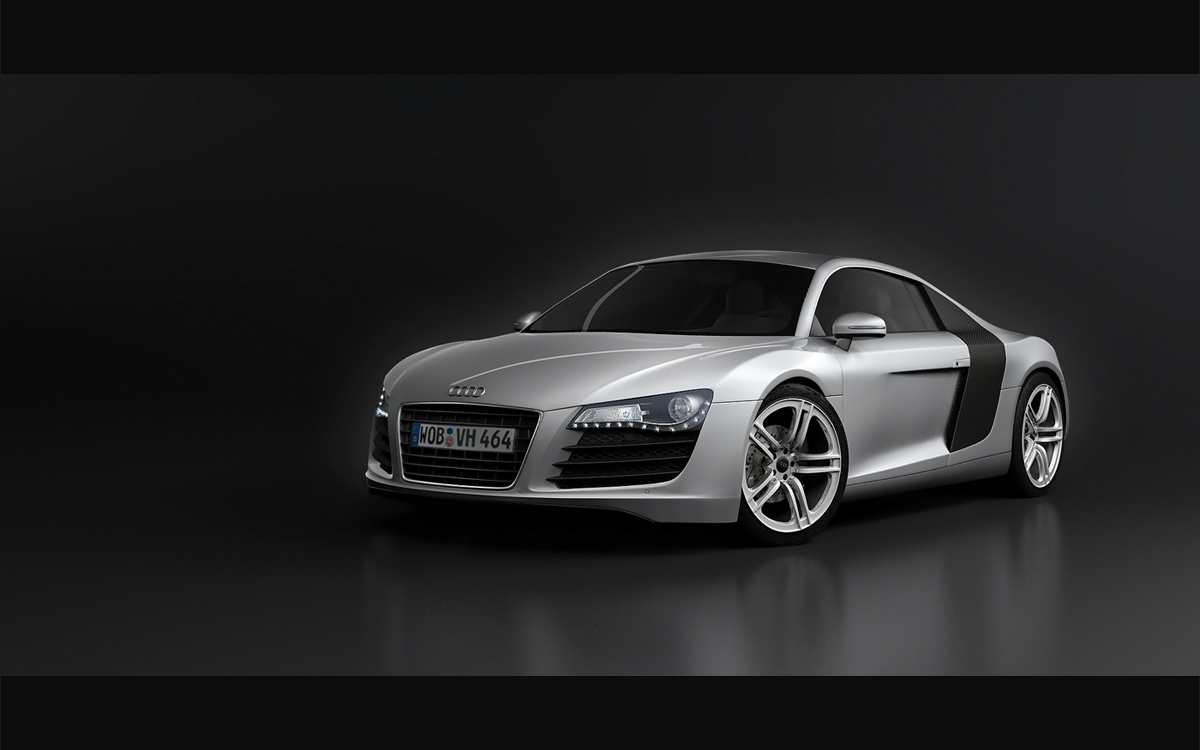
\includegraphics[width=0.8\textwidth]{audi}
    \label{fig:audi}
\end{figure}

Although one can produce very stunning imagery with a ray tracing based render engine, this  comes at a great computation cost, e.g.\ a frame from a recent computer generated Pixar's movie takes between three and eight hours to render. \cite{pixarRentime} \\
Though great computation times, major animation studios seems nowadays to be fond of ray tracing and make switches from scanline-based rendering approaches such as "REYES" which were proved stable and fast over the years to ray tracing. \cite{pixarSwitch} That points to the demands in the entertainment industry for more physically accurate imagery, but also pushes the boundaries of research in ray tracing and its computational efficiency. \cite{disneyHyperion}

% some history behind ray tracing
\subsection{The roots of ray tracing}
The first ray tracing algorithm was introduced by Arthur Appel in 1968 \cite{appel}, which idea was to shoot from the eye, one per pixel, and find the closest object blocking the path of that ray. Using the material properties and the effect of the lights in the scene, this algorithm can determine the shading of objects. \\
The next notable contribution in ray tracing was made by Turner Whitted in 1979 \cite{whitted}, who introduced natural ray technique to compute shadows as well as recursive ray tracing to handle reflective and refractive materials. \\
Other major contributions in the scene of ray tracing were made by Robert Cook in 1984 \cite{cook} and James Kajiya in 1986 \citep{kajiya} introducing distributed ray tracing and the Rendering equation respectively. But because the accompanying ray tracer does not make extensive use of these concepts, they won't be discussed in detail.

% basic ray tracing algorithm concept


%----------------------------------------------------------------------------------------
%	SECTION 2
%----------------------------------------------------------------------------------------

\section{Ray-object intersection tests}
\label{sec:isects}


%----------------------------------------------------------------------------------------
%	SECTION 3
%----------------------------------------------------------------------------------------

\section{Cameras and the image plane}
\label{sec:cameras}

%----------------------------------------------------------------------------------------
%	SECTION 4
%----------------------------------------------------------------------------------------

\section{Transformations}
\label{sec:transform}

%----------------------------------------------------------------------------------------
%	SECTION 5
%----------------------------------------------------------------------------------------

\section{Acceleration structures}
\label{sec:accel}

%----------------------------------------------------------------------------------------
%	SECTION 6
%----------------------------------------------------------------------------------------

\section{Answers to Definitions}

%----------------------------------------------------------------------------------------
%	BIBLIOGRAPHY
%----------------------------------------------------------------------------------------

\bibliographystyle{alpha}
\bibliography{references}

%----------------------------------------------------------------------------------------

\end{document}